%%%%%%%%%%%%%%%%%%%%%%%%%%%%%%%%%%%%%%%%%
% University/School Laboratory Report
% LaTeX Template
% Version 3.1 (25/3/14)
%
% This template has been downloaded from:
% http://www.LaTeXTemplates.com
%
% Original author:
% Linux and Unix Users Group at Virginia Tech Wiki 
% (https://vtluug.org/wiki/Example_LaTeX_chem_lab_report)
%
% License:
% CC BY-NC-SA 3.0 (http://creativecommons.org/licenses/by-nc-sa/3.0/)
%
%%%%%%%%%%%%%%%%%%%%%%%%%%%%%%%%%%%%%%%%%

%----------------------------------------------------------------------------------------
%	PACKAGES AND DOCUMENT CONFIGURATIONS
%----------------------------------------------------------------------------------------

\documentclass{article}

\usepackage[version=3]{mhchem} % Package for chemical equation typesetting
\usepackage{siunitx} % Provides the \SI{}{} and \si{} command for typesetting SI units
\usepackage{graphicx} % Required for the inclusion of images
\usepackage{natbib} % Required to change bibliography style to APA
\usepackage{amsmath} % Required for some math elements 
\usepackage[utf8]{inputenc}
\usepackage{tikz,pgfplots}
\usepackage[letterpaper, margin=0.5in]{geometry}
\usepackage{float}
\usepackage{enumitem}
\usepackage{gensymb}
\usepackage[hidelinks]{hyperref}
\usepackage[all]{hypcap}
\usepackage{subfloat}
\usepackage{color}
\usepackage{listings}

% Roman numerials
\pagenumbering{arabic}

\setlength\parindent{0pt} % Removes all indentation from paragraphs

%\renewcommand{\labelenumi}{\alph{enumi}.} % Make numbering in the enumerate environment by letter rather than number (e.g. section 6)

%\usepackage{times} % Uncomment to use the Times New Roman font

% for some tables
\newcommand{\specialcell}[2][c]{%
  \begin{tabular}[#1]{@{}c@{}}#2\end{tabular}}
  
\newcommand{\me}{\mathrm{e}}
\providecommand{\e}[1]{\ensuremath{\times 10^{#1}}}

\newcommand{\eqname}[1]{\tag*{#1}}

\DeclareMathOperator\erfc{erfc}

%%%%%%%%%%%% COLOR DEFINITIONS %%%%%%%%%%%%%

\definecolor{silicon}{RGB}{255,102,102}
\definecolor{oxide}{RGB}{145,150,110}
\definecolor{ioxide}{RGB}{175,180,135}
\definecolor{goxide}{RGB}{195,200,150}
\definecolor{poly}{RGB}{155,20,155}
\definecolor{spinglass}{RGB}{200,205,100}
\definecolor{n+}{RGB}{250,15,15}
\definecolor{aluminum}{RGB}{30,30,30}

%----------------------------------------------------------------------------------------
%	DOCUMENT INFORMATION
%----------------------------------------------------------------------------------------

%\title{Determination of the Atomic \\ Weight of Magnesium \\ CHEM 101} % Title

%\author{John \textsc{Smith}} % Author name

%\date{\today} % Date for the report

\begin{document}

%\maketitle % Insert the title, author and date

% If you wish to include an abstract, uncomment the lines below
% \begin{abstract}
% Abstract text
% \end{abstract}

%----------------------------------------------------------------------------------------
%	SECTION 1
%----------------------------------------------------------------------------------------

\section{Profiles \& Layout}
\subsection{}
\subsection{}
\subsection{}
\section{Process Procedures}
\subsection{Process Monitoring Measurements}

\textbf{Describe monitoring measurements that were done during processing:} \\

\textbf{Film color} - 
Film color was used during etching processes. In order to determine wheather a layer had finished etching, we used visual queues by paying attention to the color change on the films. e.g. we know aluminum etch will have finished once the silver metalish color disappeared on the wafer. \\
 
\textbf{Line Width} - 
The width of 2 um lines were measured after photolithography and after etching and PR removal to determine the amount of overetch that occured for a given layer. \\

\textbf{Thickness} -
The nanospec machine in the lab is used to measure film thicknesses. This can be done directly on our wafers or can be done on control wafers. We use control wafers in the process to measure certain film thicknesses as well as resistivities. \\

\textbf{Resistivity} - 
A four-point probe was used to measure the sheet resistance of the control wafer to monitor diffusion effects on doping concentration. \\

\textbf{Vernier} - 
Interlocking bars with slightly different spacing were produced by aligning the alignment keys of different mask layers. The offset of the bars allows the offset of the alignment between different layers to be determined very precisely. \\

\textbf{Determine whether each layer was overetched or underetched? Did you purposely
over/underetch? Why?} \\

\textbf{Field Oxide} - Overetched. This was purposely overetched to ensure process latitude. \\
\textbf{Polysilicon} - Overetched. This was overetched in order to \\
\textbf{Gate Oxide} - Overetched. This was overetched in order to keep the source/drain clear. \\
\textbf{Intermed Oxide} - Overetched. This is because we want to make sure our contact holes are open before metalization. If the contact holes are blocked by oxide, our device will not function. \\
\textbf{Aluminum} - Underetched. \\ \\ 
\textbf{Describe how the verniers are used to measure misalignment. Using diagrams may
help. Were any layers misaligned intentionally? For each pair of verniers (ACTVPOLY,
ACTV-CONT, POLY-CONT, CONT-METL), describe how far the marks
may be misaligned in terms of device function. (6 Points)} \\

\subsection{}
\subsection{}
\section{Calculations}
a) Film Thickness
\begin{figure}[H]
\centering
\begin{tabular}{c || c | c | c | c | c | c}
Layer & \specialcell{Theoretical \\ calculation \\ (nm)} & \specialcell{Experimental \\ (nm)} & \% Error & \specialcell{Linewidths \\ (photoresist) \\ (nm)} & \specialcell{Linewidths \\ (after PR Strip) \\ (nm)} & \% Overetch \\ \hline

Field Oxide & 505.8 & 477.2 & 5.65 & 2000 & 3000 & 50 \\ \hline
Polysilicon & 350 & 400 & 14 & 3628 & 4000 & 10 \\ \hline
Gate Oxide & 80.1 & 86.5 & 7.40 & 3628 & 4000 & 10 \\ \hline
Intermed Oxide & 386.3 & 320 & 17.2 & 2749 & 1869 & 47 \\ \hline
Aluminum & 800 & N/A & N/A & 2088 & 2520 & 21 \\ \hline
\end{tabular}
\caption{film thicknesses and line widths for various thin films. N/A represents data that was not available.}
\end{figure}

b) Sheet Resistance 
\begin{figure}[H]
\centering
\begin{tabular}{c || c | c }
Layer & \specialcell{Sheet Resistance \\ $\Omega/sqr$} & \specialcell{Surface Concentration \\ ($\text{cm}^{-3}$)} \\ \hline
\specialcell{ACTV after \\ Field Oxidation} & 530 & 6\e{19} \\ \hline
Polysilicon & 730 & 4\e{19} \\ \hline
\specialcell{ACTV after \\ Pre-Dep} & 5 & 5\e{22} \\ \hline
\specialcell{ACTV after \\ Drive-In} & 8 & $10^{21}$ \\ \hline
Metal & N/A & N/A \\ \hline

\end{tabular}
\caption{Surface concentrations calculated from sheet resistance using the irvin curves in jaeger (figure 4.16). The surface concentration used here is $N_B = 8\e{14}$ according to the silicon wafer resistivity. Junction depths for pre-diffusion and drive-in were calculated in Appendix \textcolor{blue}{\ref{sec:jdepth}}. For field oxide, the junction depth used was the amount of silicon consumed when growing the field oxide ($(0.46)(477\text{ nm}) = 219 \text{ nm}$). For poly and gate oxide, we calculated ($(0.46)(86.5) = 39.8$ nm) of silicon that got consumed during gate oxide growth. Therefore a junction depth of $219 + 39.8 = 258.8$ nm. Refer to Appendix \textcolor{blue}{\ref{sec:oxide}} for how to calculate oxide thickness.}
\label{fig:sheet}
\end{figure}

c) Overetch
\begin{figure}[H]
\centering
\begin{tabular}{c || c | c | c | c | c}
Layer & \specialcell{Measured Linewidth \\ (nm)} & \% Overetch & \specialcell{Theoretical \\ etch time \\ (min)} & \specialcell{Actual \\ etch time \\ (min)} & \% Overetch \\ \hline

Field Oxide &  3000 & 50 & 4.8 & 6 & 25 \\ \hline
Polysilicon &  4000 & 10 & 1.6 & $\sim2.25$ & 41  \\ \hline
Gate Oxide &  4000 & 10 & 0.87 & 0.83 & 4.6 \\ \hline
Intermed Oxide &  1869 & 47 & 3.2 &  4.5 & 41 \\ \hline
Aluminum &  2520 & 21 & 1.4 & $\sim5$ & 360 \\ \hline

\end{tabular}
\caption{Linewidth measurements and etch times used during lab. The theoretical etch times were calculated with etch rates and film thicknesses.}
\end{figure}
%%%%%%%%%%%%%%%%%%%%%%%%%%%%%%
\begin{description}[style = nextline]
\item[1) Theoretical and experimental thicknesses of field oxide, gate and intermediate 
oxides (Include orientation dependence of oxidation rate but not impurity 
dependence) (9 points)]
For details on the theoretical oxide thickness calculations see Appendix \textcolor{blue}{\ref{sec:oxide}}.
%NOTE REDO DRY OXIDE AND INCLUDE TAO OF 25nm!
\begin{figure}[H]
\centering
\begin{tabular}{c || c | c | c}
Layer & \specialcell{Theoretical \\ (nm)} & \specialcell{Experimental \\ (nm)} & \% Error \\ \hline
Field Oxide & 505.8 & 477.2 & 5.65 \\ \hline
Gate Oxide & 80.1 & 86.5 & 7.40  \\ \hline
Intermed Oxide & 386.3 & 320 & 17.2 \\ \hline
\end{tabular}
\end{figure}

\item[2) Junction depths after pre-diffusion and drive-in (theoretical, assume only 
phosphorous doping with surface concentration limited by solid solubility). You 
must consider the effect of the initial ion implantation. For pre-deposition you may 
use the box approximation, but for drive-in you must use the half-gaussian 
calculation. Why is this? (10 points)]

For details on the junction depth calculations see Appendix \textcolor{blue}{\ref{sec:jdepth}}. Also the reason we use a box approximation for the pre-diffusion is because we have a constant source profile. However, for drive-in we now have source-limited diffusion.

\begin{figure}[H]
\centering
\begin{tabular}{c || c}
Step & \specialcell{Vertical \\ junction Depth \\ (nm)} \\ \hline
Pre-diffusion & 365 \\ \hline
Drive-in & 1000 \\ \hline
\end{tabular}
\end{figure}

\item[3) Final surface concentrations of dopants, as determined from Irvin’s curves using
sheet resistance measurements made in lab. (2 points)]
Refer to Figure \textcolor{blue}{\ref{fig:sheet}}

\item[4) Plot or sketch the change of dopant profile from the silicon surface through the source-drain after each thermal step. Quantitatively label significant points such as Peak concentration, Peak Width, Junction Depth. Show movement of the Silicon-Silicon Dioxide interface and qualitatively show non-ideal effects such as dopant redistribution during oxidation. (11 points)]
The profiles were all created in Tsuprem-4 using the EE143 process flow.

\begin{itemize} 
\item Field Oxidation 
\end{itemize}
\begin{figure}[H]
\centering
\begin{tikzpicture}
\node at (5,5) {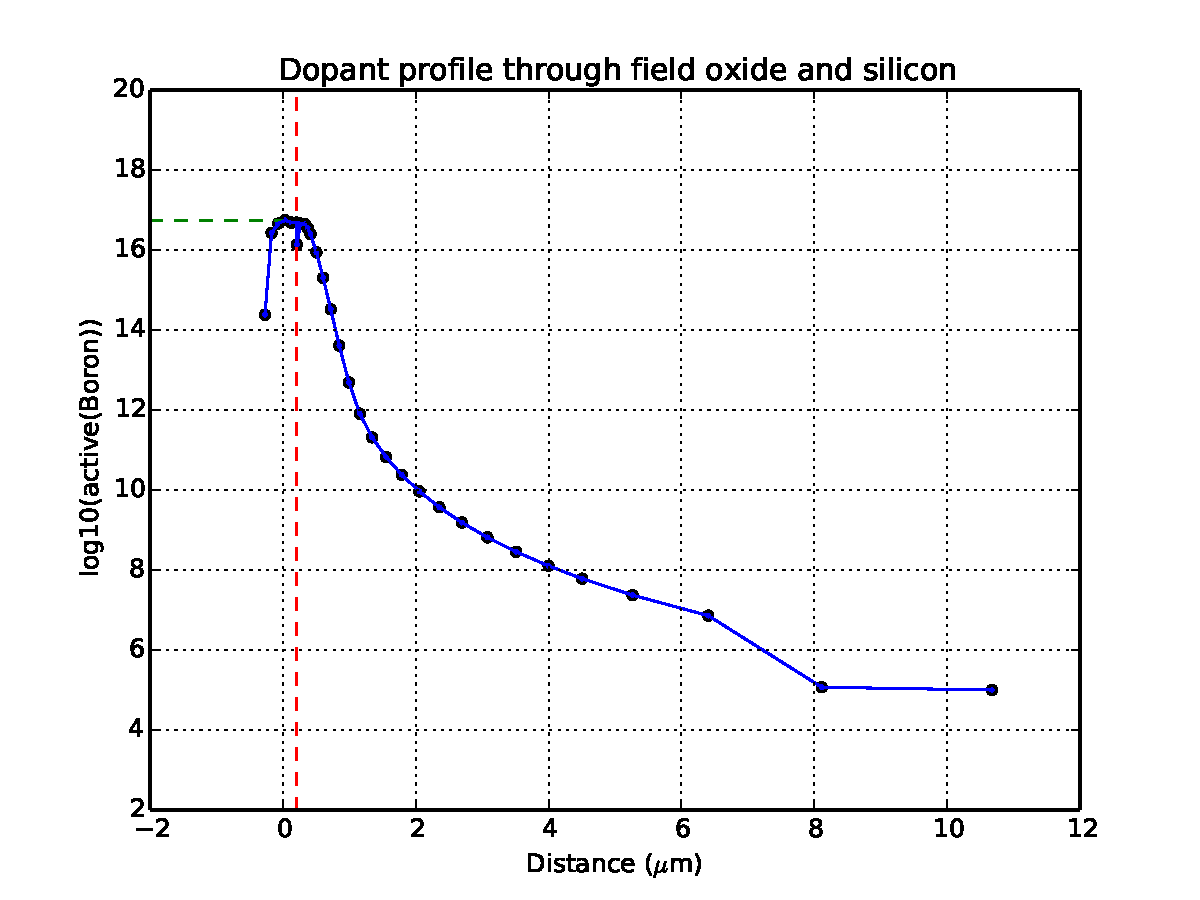
\includegraphics[width=350pt]{dope_profile/profile1.pdf}};
\node at (1.1,2.5) {\textbf{Si$\text{O}_2$}};
\node at (2.5,2.5) {\textbf{Si}};
\node at (1.0,7.6) {16.74};
\end{tikzpicture}
\caption{Dopant profile with only field oxide. The Si-Si$\text{O}_2$ interface occurs at 0.2104$\mu$m. There was about 500 nm of field oxide deposited here. The peak concentration is roughly ${10}^{16.74}$.}
\label{fig:doping1}
\end{figure}

\begin{itemize} 
\item Gate Oxidation 
\end{itemize}

\item[5) Lateral diffusion under the MOSFET gates. You may estimate. Justify estimation.
(Theoretical). (2 points)]
Using the data calculated in Appendix \textcolor{blue}{\ref{sec:jdepth}}, we see that for pre diffusion $N_0 = 10^{21}/\text{cm}^3$ and $N_B = 8\e{14}/\text{cm}^3$. Now we will use figure 4.10a [1] in the textbook and note that $N_B/N_0 \approx 10^{-7}$. Since our data goes off the graph in the figure, we will make an approximation that every multiple of 10 decrease in $N_B/N_0$ results in a vertical and lateral junction depth increase of 0.5. Using this approximation we get a vertical junction depth of 4.3 and a lateral depth of 3.8. This gives us $3.8/4.3 = 0.88$. Now from our earlier junction depth calculations we see that pre diffustion resulted in a depth of 365 nm. Thus $(365)0.88 = 321$ nm lateral junction depth for pre diffusion. For drive-in we have the same values of $N_B$ and $N_0$, but our junction depth here increased by 1000 nm. Thus $(1000)0.88 = 880$ nm.
\begin{figure}[H]
\centering
\begin{tabular}{c || c}
Step & \specialcell{Lateral \\ junction Depth \\ (nm)} \\ \hline
Pre-diffusion & 321 \\ \hline
Drive-in & 880 \\ \hline
\end{tabular}
\end{figure}


\item[6) List an estimate of the Young's modulus, Poisson ratio, and coefficient of thermalexpansion for Si$\text{O}_2$, poly-Si, and Al films as deposited. (You can find these in a table in many physics/ME textbooks, or in a web-based search.) (2 points) ]
See table below

\begin{figure}[H]
\centering
\begin{tabular}{c || c | c | c}
Material & \specialcell{Young's modulus \\ (GPa)} & \specialcell{coeff. of \\ thermal expansion \\ ($K^{-1}$)} & \specialcell{Poisson's ratio \\ (a.u.)} \\ \hline
Si$\text{O}_2$ [3]& 57(dry)-70(wet) & 5.6 $ \cdot$ 10$ ^{-7}$  & 0.17 \\ \hline
poly-Si [2]& 169 $\pm$ 6.15 & 4.6 $ \cdot$ 10$ ^{-6}$ & 0.22 $\pm$ .011 \\ \hline
Aluminum [4]& 70 & 22.2 $\cdot$ 10$ ^{-6}$ & 0.33 \\ \hline
\end{tabular}
\caption{Values were found from various journals/articles found online ([2],[3], and[4]) and many of these values are calculated for thin films of the material.}
\end{figure}


\end{description}
\section{Questions}
\begin{description}[style = nextline]
\item[1) What type of photoresist (positive or negative? I-line or G-line?) do we use in the
lab? What do I-line and G-line refer to? Briefly describe how the resist responds
to the process steps like spinning, UV light exposure and development.]
The lab uses positive photoresist. The lithography machine uses a light that has g line wavelength. The I and G lines refer to the wavelength of the light coming off the light bulb that reacts with the photoresist. G line is roughly 436nm wavelength and I line is 365nm wavelength. Photoresist is spun onto the wafer to spread it evenly over the wafer, but extreme topology and surface debris can cause excess PR in some areas and deficient PR in others. When exposed to UV light, the photo-sensitive part of the polymer activates changing it into an organic acid, whereas unexposed PR remains unchanged. When dipped into the PR developer, the organic acid form of the PR dissolves whereas the polymer form remains on the wafer, leaving a layer PR that masks certain areas of the wafer.

\item[2) What is the purpose of baking the wafers at 120 $\degree$C before depositing HMDS? What
is the purpose of the 90 $\degree$C bake after spinning on photoresist? What happens if the
soft bake is too hot and too long (say 120 $\degree$C, 5 minutes)?]
The purpose of baking the wafers at 120$\degree$C before depositing HMDS is to remove excess environmental moisture that has accumulated on the wafer. The purpose of the 90$\degree$C bake after spinning on photoresist is to evaporate the solvent and make it less sticky. If the soft bake is too long, the photoactive component of the PR may start to decompose and the PR may become less soluable in the developer. 

\item[3) What is the purpose of hard bake? What happens if we skip this step? What may
happen if the bake is done at a temperature above 120 $\degree$C (say 200 $\degree$C)?]
The purpose of the hard bake is to cross-polymerize the PR, making it less permeable to chemicals, more adhesive, and physically harder. If this step is skipped, subsequent etching and similar steps have a chance of penetrating the PR, making the mask meaningless. If the bake is done at a temperature above 120$\degree$C, the PR will start to become brittle, resulting in cracks that would also make the masking step meaningless.

\item[4) We do lithography steps under yellow light only. What is the consequence if we
expose the wafers to fluorescent light before development? What if we expose
them to fluorescent light after development? Would red light damage your process?]
If the fluorescent light happens to be near the wavelength of the g-line, it will react with the photoresist and make it soluble. Since there is no mask over the wafer at that time, it will make all the photoresist souble which will cause the developer to remove all the photoresist. If it were exposed after developement, it will still make the remaining photoresist soluble, but since we have already done developement, there is no risk of the remaining photoresist coming off (unless we were to dip it in the developer again).

\item[5) What are the differences between wet and dry oxidation that lead us to use one for
the gate oxide and one for the field/intermediate oxide? What is the purpose of
annealing in nitrogen after oxidation?]
Wet oxidation has a higher growth rate but a tendency to create dangling bonds and a lower density oxide, making it more suitable for the thick field/intermediate oxide. Dry oxidation is much slower but creates a higher density oxide with fewer dangling bonds, making it more suitable for creating the thin gate oxide that is critical in device performance. The purpose of annealing in nitrogen is to allow the silicon atoms to diffuse and repair damage done by oxidization. 

\item[6) How do you determine etching time using theoretical etch rate in literature? List
two ways to determine etch time empirically from lab measurements, when you
etch the layers. (Hint: these methods include visual cues.). How close are the
experimental and the theoretically calculated values?]

\item[7) Before n+ deposition (prior to SOG spinning), we clean in Piranha but not in HF.
Before gate oxidation, we clean in both. Why the difference?]
For n+ deposition, we are depositing PSG (a phosphorate-doped oxide) on top of the wafer for diffusion. The presence of a native oxide on the surface serves as a barrier material between the PSG and the silicon, preventing unwanted inter-diffusion effects. However, for growing a high-quality gate oxide, the poor-quality native oxide will adversely affect results, thus it must be removed with an HF dip.

\item[8) Why is 5:1 BHF (5:1 N$\text{H}_4$F:HF) used for etching features in the oxide while 10:1
BHF is used for cleaning and spin-on-glass stripping? Why buffered HF? ]
We use buffered HF because normal HF etches way too quickly and tends to peel off photoresist as well. Using buffered HF allows for more controllable and constant etching which allows for good process control. According to the process flow, spin on glass etches at 470 nm/sec in 10:1 BHF while thermally grown oxide etches at 100nm/sec in 5:1 BHF. If we had used 5:1 BHF for the spin on glass, it would etch way to quickly and be difficult to control.

\item[9) What would happen if we skipped the HF dip before metallization? ]
Skipping the HF dip before metallization would result in a thin layer of native oxide at the Al-Si interface, causing poor contact with the devices on the wafer.

\item[10) What is etch selectivity? ]
Etch selectivity is the relative difference in etch rates for given materials on the wafer. Ideally, the etch should be highly selective towards the material to be etched and thus etch it the fastest whereas other material, like the PR, should etch much more slowly.

\item[11) Why do we first use the roughing pump and then the diffusion pump when pumping
down the aluminum deposition system? Why must the foreline pressure be kept
below 100 mTorr?]

\item[12) What is the Al etchant composed of? What happens if you use it at room
temperature? What is the purpose of sintering? What will result if sintering step is
skipped? What happens if sintering temperature is too hot or too low?]
Al etchant has a composition of 80\% Phosphoric acid, 10\% H2, 5\% acetic acid, and 5\% nitric acid. It etches much more slowly at room temperature then at 50 degC. Sintering allows the aluminum and silicon to interdiffuse, resulting in a good contact, as well as allowing hydrogen to diffuse into the oxide and tie up dangling bonds. If the sintering step is skipped, the contact may be poor. If the sintering temperature is too hot, the eutectic Al-Si system will melt. If the sintering temeperature is too low, the contact resistance between the aluminum and silicon will be too high.


\item[13) Briefly explain the mechanism of Xe$\text{F}_2$ etching. Is the etch isotropic or
anisotropic? In an integrated CMOS/MEMS process, is there any consequence to
using KOH instead of Xe$\text{F}_2$ for etch?]
XeF2 gas is absorbed by the silicon surface, where it breaks down into xenon and fluoride gas. The fluoride gas reacts with the silicon to form SiF2 gas, and both the xenon and SiF2 gas are released back into the air. XeF2 etching is isotropic. Using KOH as an etchant instead of XeF2 has two consequences. First, it is anisotropic and therefore less efficient at undercutting the beam. Secondly, it is a wet etch and liquid etchants can cause the freed structure to stick to the substrate. 

\item[14) . What would happen if a thick oxide film was left on the wafers as it went into the
Xe$\text{F}_2$ etching step? ]
Since XeF2 is highly selective against SiO2, the structure would not be freed as the etchant would not be able to etch through the oxide film to the silicon below.

\item[15) Identify two of the 11 major processing steps that are unnecessary to fabricate a
functional oxide cantilever beam. Why are they unnecessary?]
Gate oxidation and S/D deposition are unnecessary to fabricating a functional oxide cantilever beam. The cantilever requires no gate so any gate oxide grown during this step must later be removed, and doping plays no part in the functioning of a cantilever device, so S/D deposition can also be skipped.

\end{description}

\section{Bonus Questions (up to 10 Points)}
\begin{description}[style = nextline]
\item[1) Simulate the 143 process flow in Tsuprem4 (8 points) (updated on 11/20/14, you
only need to simulate the NMOS LDD example available online (i.e., s4ex4a, -b, -
c.inp))]
I ran the files provided to us by Wei-chang on one of the eecs linux servers that had tusprem-4 installed. I only changed input/output directories in the script files to get them to work properly. Here is the resulting figure that is plotted after compiling and running the example NMOS.
\begin{figure}[H]
\centering
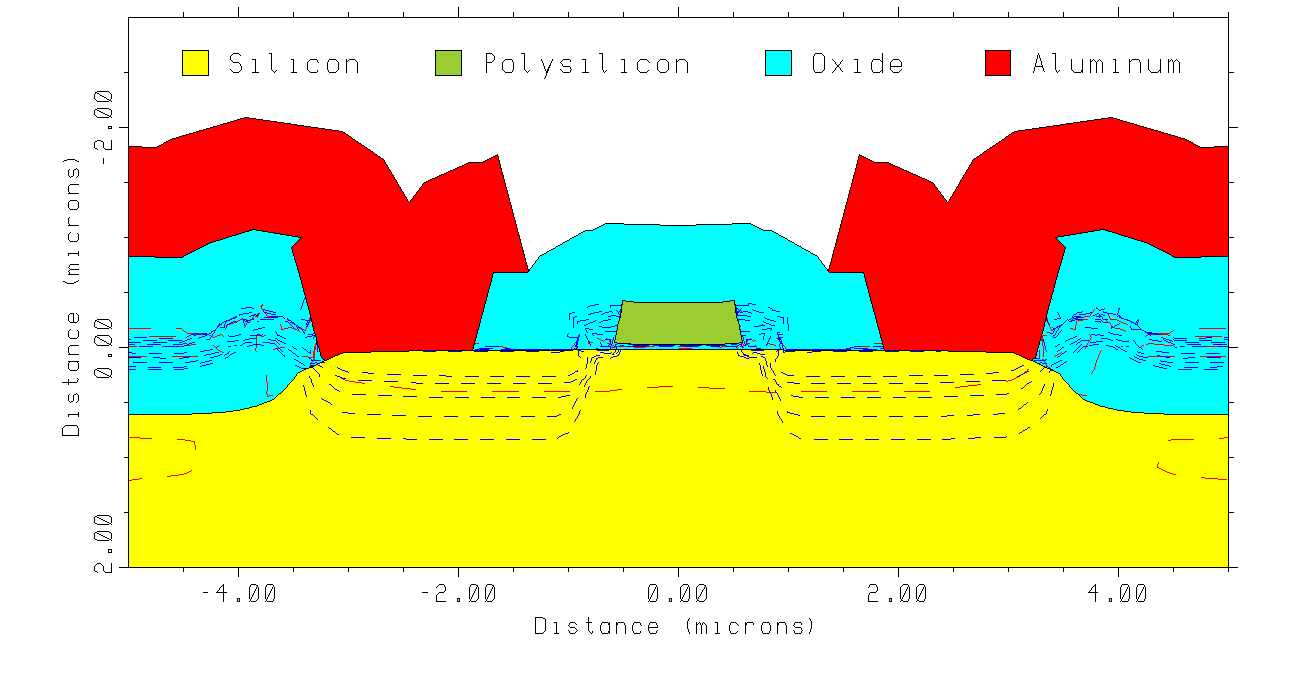
\includegraphics[width=325pt]{calcs/bonus1.png}
\caption{tsuprem4 generated NMOS example process}
\end{figure}

\item[2) Describe an alternate method for doing one of the process steps (i.e. LOCOS instead
of Field Oxide, Sputtering instead of Evaporation, etc) and the tradeoffs.]
\end{description}

\section{Appendix}

\subsection{Oxide Thickness calculations}
\label{sec:oxide}
Film thickness calculation for oxides:
\begin{equation}
X_{ox} = \frac{0.5B}{B/A}\Big[\sqrt{1 + \frac{4}{B}(\frac{B}{A})^2(t + \tau)} - 1\Big]
\end{equation}
\begin{equation}
\tau = \frac{{X_i}^2}{B} + \frac{X_i}{B/A}
\end{equation}
where
\begin{align*}
B/A = D_o\me^{\frac{-E_a}{kT}} (\text{Use table 3.1 [1] to find }E_a \text{and } D_o) \\
B = D_o\me^{\frac{-E_a}{kT}} (\text{Use table 3.1 [1] to find }E_a \text{and } D_o) \\
t = \text{Time of oxide growth} \\ 
\tau = \text{Time of initial oxide growth already present} \\
X_i = \text{length of initial oxide growth}
\end{align*}

Example: Calculated oxide thickness of Intermed Oxide: \\
Given: 5 min dry oxidation at $1050\degree$C and 12 + 25 min wet oxidation annealing at $1050\degree$C, calculate oxide growth. \\

First we consider the 5 min dry oxidation. Using table 3.1 [1] for a $<100>$ Silicon, and using dry oxidation, we see that for the linear rate constant (B/A), $E_A = 2.00$ eV and $D_o = 3.71\e{6} \, \mu$m/hr. For the parabolic rate constant (B), $E_A = 1.23$ eV and $D_o = 772\, \mu$m/hr. \\ \\
Using an arrhenius equation where $k =$ Boltzmann's constant, and $T = $ temperature. 
\begin{align*}
B/A &= D_o\me^{\frac{-E_A}{kT}} = 3.71\e{6}\me^{\frac{-2.00*1.602\e{-19}}{1.38\e{-23}(1050\degree\text{C} + 273)}} = 0.0887 \mu\text{m/hr} \\
B &= D_o\me^{\frac{-E_A}{kT}} = 772\me^{\frac{-1.23*1.602\e{-19}}{1.38\e{-23}(1050\degree\text{C} + 273)}} = 0.0159 \,{\mu\text{m}}^2\text{/hr}
\end{align*}
Since there is no initial oxide here, $\tau = 0$,
\begin{align*}
X_{ox} = \frac{0.5B}{B/A}\Big[\sqrt{1 + \frac{4}{B}(\frac{B}{A})^2(t + \tau)} - 1\Big] = \frac{0.5 (0.0159)}{0.0887}\Big[\sqrt{1 + \frac{4}{0.0159}(0.0887)^2(\frac{5\text{min}}{60\text{min/hr}} + 0)} - 1\Big] \approx 7.11 \, \text{nm}
\end{align*}

Now after this dry oxidation, we have a 37 minute wet oxidation at $1050 \degree$C. Using table 3.1 [1] again, but this time using the constants that apply for wet oxidation,

\begin{align*}
{B/A}_{\text{wet}} &= D_o\me^{\frac{-E_A}{kT}} = 9.70\e{7}\me^{\frac{-2.05*1.602\e{-19}}{1.38\e{-23}(1050\degree\text{C} + 273)}} = 1.50 \mu\text{m/hr} \\
B_{\text{wet}} &= D_o\me^{\frac{-E_A}{kT}} = 386\me^{\frac{-0.78*1.602\e{-19}}{1.38\e{-23}(1050\degree\text{C} + 273)}} = 0.411 \,{\mu\text{m}}^2\text{/hr}
\end{align*}

This time we do have an initial oxidation time $\tau$ because of the dry oxidation we did in the previous step. Here $X_i$ is the oxide length we calculated for the dry oxidation growth,

\begin{align*}
\tau = \frac{{X_i}^2}{B_{\text{wet}}} + \frac{X_i}{{B/A}_{\text{wet}}} = \frac{0.00711^2}{0.411} + \frac{0.00711}{1.50} \approx 0.00488 \text{hrs}
\end{align*}

And finally our oxide growth is,
\begin{align*}
X_{ox} = \frac{0.5B}{B/A}\Big[\sqrt{1 + \frac{4}{B}(\frac{B}{A})^2(t + \tau)} - 1\Big] = \frac{0.5 (0.411)}{1.50}\Big[\sqrt{1 + \frac{4}{0.411}(1.50)^2(\frac{(12 + 25)\text{min}}{60\text{min/hr}} + 0.00488 \text{hrs})} - 1\Big] \approx 386.3 \, \text{nm}
\end{align*}

\subsection{Junction Depth Calculations}
\label{sec:jdepth}
Junction depth calculation for box approximation (limited-source diffusion):
\begin{equation}
x_j = 2\sqrt{Dt \ln{(N_o/N_B)}}
\end{equation}
and for a half gaussian (constant-source diffusion):
\begin{equation}
x_j = 2\sqrt{Dt}\erfc^{-1}{(N_B/N_o)}
\end{equation}
where,
\begin{align*}
D &= D_o\me{\frac{-E_A}{kT}} \,\,\text{(Diffusion coefficient)} \\ 
t &= \text{time of diffusion} \\
N_B &= \text{Background impurity concentration} \\ 
N_o &= \text{Surface concentration limited by solid solubility}
\end{align*}

Example: Calculate the junction depth after pre-diffusion and drive in. \\
According to the process flow [5], our silicon wafer has a resistivity of about 14-16 ohm-cm. From the same process flow we know that we had a phosphorus doped, solid solubility limited constant diffusion at $1050\degree$C. Using figure 4.6 [1] we see that at a temperature of $1050\degree$C our phosphorus surface concentration $N_o \approx 10^{21}$/$\text{cm}^3$. Now using the Resistivity of our wafer and figure 4.8 [1], we see that we have an impurity concentration $N_B \approx 8\e{14}/\text{cm}^3$. \\ \\
Using table 4.1 [1], we can calculate our diffusion coefficient. Note that pre-diffusion was done at $1050\degree$C for 5 minutes.
\begin{align*}
D &= D_o\me{\frac{-E_A}{kT}} = 10.5 \,\text{cm}^2/\text{sec}\,\, \exp{(\frac{-3.69*1.602\e{-19}}{1.38\e{-23}(1050 + 273)})} = 9.11\e{-14} \, \text{cm}^2/\text{sec}
\end{align*}
Now we can plug everything into our solid solubility limited box approximation equation:
\begin{align*}
x_j = 2\sqrt{Dt}\erfc^{-1}{(N_B/N_o)} = 2\sqrt{(9.11\e{-14})(300\text{sec})} \erfc^{-1}{(8\e{14}/10^{21})} \approx 365 \,\text{nm}
\end{align*}

Now for drive-in we kept the temperature the same, $1050\degree$C, but kept the wafer inside the furnace for 37 minutes (2220 seconds). Also we can no longer assume a simple box approximation, we must use a half gaussian; this means that our surface concentration is going to change with drive-in. \\\\
We will use the following equation,

\begin{equation}
N_B = (Q/\sqrt{\pi D_2t_2})\exp{(-(\frac{x_j}{2\sqrt{D_2t_2}})^2)}
\end{equation}

where Q is the does rate,
\begin{equation}
Q = 2N_o\sqrt{D_1t_1/\pi}
\end{equation}

Combining the two equations and noting that $D_1 = D_2$ because we are using the same temperature, $1050\degree$C, for both pre-diffusion and drive-in ($t_1$ is the pre-diffusion time and $t_2$ is the drive in time),

\begin{align*}
N_B = (2N_o/\pi)\sqrt{\frac{t_1}{t_2}}\exp{(-(\frac{x_j}{2\sqrt{D_2t_2}})^2)}
\end{align*}
Solving this for $x_j$ yields,
\begin{align*}
x_j = 2\sqrt{D_2t_2\ln{\big((2N_o/\pi N_B)(\sqrt{t_1/t_2})\big)}} = 2\sqrt{(9.11\e{-14})(2220)\ln{\big((2(10^{21})/\pi (8\e{14}))(\sqrt{300/2220})\big)}} \approx 1000 \,nm
\end{align*}

\subsection{Dopant Profiles.}
\begin{itemize}
\item Field Oxide
\end{itemize}
According to the EE143 process flow, There was an initial blanket implant of B11 3E12$\text{cm}^{-3}$ on our $<100>$ wafer. Also our wafer had a resistivity of 14-16cm which corresponds to a background concentration of about 8E14$\text{cm}^{-3}$. Now for the field oxide, we used 5-80-5 minute dry,wet,dry oxidation to create about 500 nm of oxide. Putting all this information into Tsuprem-4 generates the plot in Figure \textcolor{blue}{\ref{fig:doping1}}. \\ \\
Script file: 
\begin{verbatim}
$ field oxide

$ Initialization 
Initialize <100> material=silicon Phosphorus=8e14 width=1.5 dX=0.005

$ Blanket implant here
Implant B11 Energy=60 Dose=3e12

$ 5-80-5 oxidation
Diffusion Time=5 Temperature=1000 DryO2
Diffusion Time=80 CONTINUE Temperature=1000 WetO2
Diffusion Time=5 CONTINUE Temperature=1000 DryO2

$ plotting
Select z=log10(active(boron))
Plot.1d
Print.1d
\end{verbatim}

\begin{itemize}
\item Gate Oxide
\end{itemize}



%----------------------------------------------------------------------------------------
%	SECTION 5
%----------------------------------------------------------------------------------------
\section{References}
\begin{enumerate}
\item Jaeger, Richard. \textit{Introduction to microelectronic fabrication}. New Jersey: Prentice Hall, 2002. Print.
\item Sharpe, William N., Bin Yuan, and Ranji Vaidyanathan. Measurements of Young's Modulus, Poisson's ratio, and Tensile Strength of Polysilicon. Publication no. 1. Nagoya: IEEE, 1997. Web.
\item Kim, Min. "Influence of Substrates on the Elastic Reaction of Films for the Microindentation Tests." Thin Solid Films 283 (1996): 15. Web.
\item Chinmulgund, M. "Effect of Ar Gas Pressure on Growth, Structure, and Mechanical Properties of Sputtered Ti, Al, TiAl, and Ti3Al Films." Thin Solid Films 270.1-2 (1995): 260-63. Web.
\end{enumerate}

%----------------------------------------------------------------------------------------
%	SECTION 6
%----------------------------------------------------------------------------------------

% Nothing right now

%----------------------------------------------------------------------------------------
%	BIBLIOGRAPHY
%----------------------------------------------------------------------------------------

\bibliographystyle{apalike}

\bibliography{sample}

%----------------------------------------------------------------------------------------


\end{document}

